%% paper.tex — ACM eEnergy 2027 Fall submission draft (or PES General Meeting November
%% fallback). Double-blind review copy: sigconf + review + anonymous.
%% Source of truth for content is paper.md; keep the two in sync by hand (paper.md is
%% easier to edit/diff, this file is what actually compiles). Converted from paper.md
%% 2026-09-12, second full draft (Related Work written+cited, n=3 replication on the two
%% flagship result pairs, Tables 1-6 + Figures 1-2 added).
\documentclass[sigconf,review,anonymous]{acmart}
\usepackage{enumitem}
\setlist[itemize]{itemsep=0.5pt,topsep=2pt,parsep=0pt,partopsep=0pt}
\setlength{\textfloatsep}{3pt plus 1pt minus 1pt}
\setlength{\floatsep}{2pt plus 1pt minus 1pt}
\setlength{\intextsep}{3pt plus 1pt minus 1pt}
\setlength{\abovecaptionskip}{2pt}
\setlength{\belowcaptionskip}{0pt}

\AtBeginDocument{%
  \providecommand\BibTeX{{Bib\TeX}}}

%% Rights-management placeholders — fill in from the rights-confirmation email after
%% acceptance. Not needed for the anonymous review submission.
\setcopyright{acmlicensed}
\copyrightyear{2027}
\acmYear{2027}
\acmDOI{XXXXXXX.XXXXXXX}
\acmConference[eEnergy '27]{ACM eEnergy 2027 Fall: 17th ACM International Conference on
  Future and Sustainable Energy Systems}{TBD 2027}{TBD}
\acmISBN{978-1-4503-XXXX-X/2027/TBD}

\begin{document}

\title{Where Admission Gating Works: Peak-Shaving for Prefill/Decode-Disaggregated LLM Serving}

\author{Anonymous Author(s)}
\affiliation{%
  \institution{Anonymous Institution}
  \country{}
}

\begin{abstract}
Utility demand caps are billed on a rolling-window average, not instantaneous power --- a
structural fact that lets a no-storage system defer admission rather than shed load to stay
under a cap, so long as it can predict the marginal energy cost of each request before
admitting it. We build such an admission gate for LLM-serving fleets and validate it on real
8$\times$4090 hardware, then ask whether it can be made more effective by exploiting real
prefill/decode (P/D) disaggregated serving: instead of one combined fleet-power budget, track
independent power budgets for the prefill pool and the decode pool, calibrated against real
(not colocated-contaminated) per-token energy measurements. The disaggregated design is not
uniformly better --- it is \emph{selectively} better, and reveals why: admission gating can
only control requests before they start, so it shaves prefill-pool peak power substantially
(18.0\% under closed-loop arrivals, 24.3\% under Poisson arrivals, at our flagship cap,
replicated $n{=}3$) but barely touches decode-pool peak power (1.2--5.7\% across every cap and
arrival pattern tested), because decode power is dominated by already-in-flight generation
streams the gate cannot retroactively throttle. A controlled concurrency sweep confirms the
mechanism directly: decode-GPU power is dominated by an idle-to-busy step (a jump of
${\sim}233$~W from 0 to 2 concurrent streams) with only a small, sub-linear dependence on load
thereafter ($+13\%$ from 2 to 32 concurrent streams) --- meaning no admission-side mechanism,
however aggressive, can shave decode power much further without idling the decode instance
entirely. We further show the prefill-side effect is a real, monotonic power/latency tradeoff
(a 4-point cap sweep, 18.0--34.9\% peak-power reduction for 10.95--20.9~s mean TTFT), and that
it is robust to arrival pattern, replicated $n{=}3$ at our flagship cap: Poisson open-loop
arrivals reproduce the same qualitative asymmetry, but the same cap costs roughly $10\times$
more latency there than under closed-loop arrivals ($+9.2$~s mean TTFT under closed-loop vs.\
$+88.7$~s under Poisson). Translating the facility-wide (combined-pool) peak reduction into
real demand-charge terms at typical U.S.\ commercial rates yields a 12.4\% cut in the
billing-relevant peak, which we report as a preliminary estimate rather than a validated bill
saving, since our measurement window is far shorter than the 15-minute interval real utility
billing uses. Building this system surfaced and fixed four real bugs --- three in
the admission gate itself (a token-counting units mismatch, a reservation-release timing
error, and an estimator-poisoning health check) and one in our own measurement harness
(silently dropped, uncounted request failures under open-loop arrivals) --- each diagnosed
from first principles and confirmed fixed by re-validation, which we report as part of the
paper's honest empirical record rather than omitting.
\end{abstract}

\maketitle

\section{Introduction}

Data centers running LLM inference increasingly face utility-imposed peak power demand
charges or hard caps, and battery/storage-backed peak shaving is not always available or
economical to deploy alongside GPU fleets. Utility billing for peak demand is not based on
instantaneous power draw, however --- it is based on the highest \emph{rolling-window
average} over a billing interval, commonly 15 minutes. This creates room for a no-storage
mechanism: an admission-control layer that defers request admission just long enough to keep
the trailing window's average power under a cap, exploiting the averaging window as a
``virtual battery'' that needs no physical energy storage at all.

We design, implement, and validate such a mechanism (\S\ref{sec:colocated}), then investigate
whether it can be made more effective under a serving architecture that is rapidly becoming
common in production LLM deployments: prefill/decode (P/D) disaggregation, where the
compute-bound prefill phase and the memory-bandwidth-bound decode phase of inference run on
physically separate GPU pools (\S\ref{sec:disaggcalib}), connected by a KV-cache transfer
mechanism (we use vLLM's \texttt{NixlConnector}). Disaggregation is usually motivated by
throughput and tail-latency isolation; we ask a different question: does it also change how
\emph{effective} peak-shaving admission gating is, and if per-pool budgets reveal something a
single combined fleet budget cannot?

\textbf{Our findings, summarized:}

\begin{enumerate}[leftmargin=*]
  \item The admission gate, validated first on colocated (non-disaggregated) serving, works:
    it measurably reduces peak power with a real, quantified tail-latency cost, and has a
    structural limit under sustained overload that we identify but do not solve in this paper
    (\S\ref{sec:limit}).
  \item Splitting one combined power budget into independent per-pool budgets under real P/D
    disaggregation does not just match the colocated result --- it \emph{reveals an asymmetry
    the colocated design cannot see}: admission gating shaves prefill-pool peak power far
    more effectively than decode-pool peak power, at every cap aggressiveness and arrival
    pattern we tested (\S\ref{sec:disagggate}).
  \item This asymmetry has a clean mechanistic explanation, confirmed by a dedicated
    controlled experiment: decode-GPU power is dominated by whether the GPU is doing
    \emph{any} decode work at all, with only a small, sub-linear dependence on how much
    (\S\ref{sec:concurrency}). Since admission gating can only prevent \emph{new} work from
    starting, it has almost no lever on a pool that is rarely, if ever, fully idle.
  \item The prefill-side effect is a genuine, monotonic, tunable power/latency tradeoff, not
    a single operating point (\S\ref{sec:tradeoff}), and it is qualitatively robust to
    arrival pattern, though not quantitatively --- the same cap costs an order of magnitude
    more latency under Poisson arrivals than under closed-loop arrivals (\S\ref{sec:poisson}).
\end{enumerate}

\textbf{What this paper contributes, stated plainly.} The admission-control mechanism itself
--- deferring requests against a rolling-window power budget rather than shedding them --- is
not a new algorithm; it is a direct application of a long-standing demand-response idea
(\S\ref{sec:related}) to a new workload. We do not claim algorithmic novelty for the gate.
What we claim is empirical: (1) an end-to-end, real-hardware validation of that mechanism under
real prefill/decode-disaggregated LLM serving, not a simulation or a colocated proxy for it;
(2) a specific, previously unreported finding that the mechanism's effectiveness is sharply and
consistently asymmetric between the prefill and decode pools, together with a controlled
experiment that pins down the mechanistic cause (\S\ref{sec:concurrency}); and (3) an honest
account of where this leaves the technique --- a genuine power/latency tradeoff on the prefill
side (\S\ref{sec:tradeoff}), a structural limit under sustained overload it does not solve
(\S\ref{sec:limit}, \S\ref{sec:poisson}), a preliminary but directly relevant translation into
demand-charge economics (\S\ref{sec:cost}), and the real bugs found and fixed while getting
there (\S\ref{sec:bugs}, \S\ref{sec:poisson}). We report this as an honest empirical systems
paper on that basis: real hardware throughout, explicit statistical caveats
(\S\ref{sec:discussion} discusses exactly what is and is not yet replicated), and full
transparency about what remains open, because we believe that diagnostic and empirical record
is itself the useful output for anyone building or evaluating similar admission-control
mechanisms --- not a new algorithm to adopt.

\section{Background and Related Work}
\label{sec:related}

\textbf{Demand response and peak shaving for data centers.} Exploiting the gap between
instantaneous and billed (averaged) power is a long-standing idea in data center power
management. Fan et al.~\cite{fan2007warehouse} first showed data centers rarely draw their
provisioned peak, enabling power oversubscription; a line of work since has proposed workload
shifting and capacity modulation to cap or smooth billed electricity cost directly, including
bill-capping algorithms that enforce a monthly budget while maximizing
throughput~\cite{zhang2012capping}. Our admission gate is a mechanism in this tradition --- a
no-storage, workload-side lever rather than a storage-side one --- applied to a workload (LLM
inference) this literature has only just begun to consider explicitly: a contemporaneous
paper~\cite{du2026tokens} proposes model-quantization as a demand-response flexibility lever
for LLM-serving data centers, complementary to (and combinable with) the admission-side lever
we study here.

\textbf{Prefill/decode disaggregation.} Disaggregating the compute-bound prefill phase from
the memory-bandwidth-bound decode phase of LLM inference onto separate hardware pools is now
a well-established systems technique, motivated by throughput and tail-latency isolation:
DistServe~\cite{zhong2024distserve} co-optimizes per-phase parallelism and placement against
phase-specific SLOs; Splitwise~\cite{patel2024splitwise} shows the two phases have distinct
power profiles and that decode can run efficiently on lower-power hardware;
Mooncake~\cite{qin2025mooncake} adds a KVCache-centric disaggregated scheduler tuned for real
production traffic. We build on this line of work directly --- our disaggregated serving
stack uses NVIDIA's NIXL transport library~\cite{nvidia2025nixl} via vLLM's
\texttt{NixlConnector}, and vLLM's \texttt{PagedAttention}~\cite{kwon2023pagedattention} as
the underlying serving engine --- but ask a different question than throughput or tail
latency: whether disaggregation changes what an \emph{admission-control} mechanism, not a
routing or placement mechanism, can achieve, and we are not aware of prior work connecting
P/D disaggregation to peak-power demand shaping specifically.

\textbf{Power-aware LLM serving.} A growing body of work characterizes and controls LLM
inference energy directly. Ma et al.~\cite{ma2026illusion} find that GPU frequency capping
during decode is far less effective than commonly assumed once phase-specific behavior is
accounted for --- a finding that resonates with, though is mechanistically distinct from, our
own result that decode power is difficult for an \emph{admission-side} (rather than
frequency-side) lever to move. GreenLLM~\cite{liu2025greenllm} uses SLO-aware dynamic
frequency scaling to cut serving energy without violating latency targets, operating at the
GPU-clock level rather than the admission level. Vellaisamy et
al.~\cite{vellaisamy2026characterization} propose a decomposed request/token energy model
(fixed prefill/setup cost plus marginal per-token decode cost) for characterizing LLM
inference energy on real GPU platforms --- the same two-term structure our own
marginal-energy estimator uses for admission decisions, developed independently and validated
here specifically under both colocated and disaggregated serving. None of this line of work,
to our knowledge, targets peak \emph{demand} (as opposed to total energy) directly, or
investigates disaggregation's effect on a peak-shaving mechanism specifically.

\textbf{Power-aware routing.} Our admission gate is designed to sit in front of, and be
independent of, a fleet's routing policy. We validate this independence against a companion
line of our own work~\cite{ghodsi2011drf, anonymous2026routing} that develops a provably
Pareto-safe power-aware routing policy (extending Dominant Resource
Fairness~\cite{ghodsi2011drf} with a reactive power dimension) for the \emph{same} class of
GPU-serving fleets; that paper addresses which replica should serve an admitted request, this
one addresses whether and when to admit it at all --- the two mechanisms are complementary
and, as \S\ref{sec:crosspolicy} shows empirically, compose without interference.

\section{The Colocated Peak-Shaving Admission Gate}
\label{sec:colocated}

\textbf{Experimental setup, used throughout this paper unless noted otherwise.} All hardware
results are on a single node with 8$\times$ NVIDIA RTX 4090 (24GB), serving
Qwen2.5-Coder-7B-Instruct via vLLM 0.23.0. Power is sampled per-GPU via NVML at 20~Hz (50~ms
interval) and aggregated to the relevant pool. Workload is generated from ShareGPT
conversational traces, single-turn, with a 15\% ``whale'' mix of long (44--50k character)
prompts injected among otherwise short conversational prompts, and a 1024-token generation
cap --- this mix is the same one used throughout our companion routing
work~\cite{anonymous2026routing} and is designed to stress both prefill (via whales) and
decode (via sustained short-prompt throughput) realistically rather than in isolation. Two
arrival patterns are used: \emph{closed-loop} (fixed concurrency, a new request replaces each
completion) and \emph{Poisson open-loop} (exponentially-distributed inter-arrival times at a
fixed target rate) --- \S\ref{sec:bugs} and \S\ref{sec:poisson} discuss why both matter.
Request timeout (client-side) is 180~s for colocated-gate batteries and 300~s for
disaggregated-gate batteries --- raised proactively, based on \S\ref{sec:crosspolicy}'s
aggressive-cap demonstration already showing that a tight cap could otherwise produce
spurious client-timeout failures rather than genuine slow completions.

\subsection{Design}

The gate sits strictly in front of an existing router's routing decision (any routing policy
--- we pair it with a DRF-style policy from our own prior work, chosen for being
routing-policy-independent in its effect, confirmed in \S\ref{sec:crosspolicy}) and decides
only \emph{whether/when} to admit a request, never \emph{which} replica serves it. A
\texttt{PowerBudget} tracks a rolling window of fleet-power samples; admission is gated on
whether admitting a request's estimated marginal energy cost would push the trailing window's
average over a configured cap. The estimator is two-term: $\mathit{marginal\_energy\_j} =
\mathit{prompt\_tokens} \times \mathit{j\_per\_prefill\_token} + \mathit{expected\_decode\_tokens}
\times \mathit{j\_per\_decode\_token}$, with \texttt{expected\_decode\_tokens} from a live
exponential moving average of realized response length (not a static \texttt{max\_tokens}
assumption, which we found overestimates typical output length by roughly $3\times$ on our
target workload). A reservation ledger closes a time-of-check-to-time-of-use race: several
requests admitted within the same power-measurement interval could otherwise each pass
against the same stale reading and collectively overshoot the cap.

\subsection{Prefill/decode energy calibration (colocated)}
\label{sec:coloc-calib}

Calibrating \texttt{j\_per\_prefill\_token} and \texttt{j\_per\_decode\_token} on colocated
serving is harder than it first appears, because prefill and decode share the same GPU and
the same batch --- a trial-level regression across ${\sim}600$ collected trials failed
outright, producing a physically-impossible \emph{negative} decode coefficient (idle power
and trial duration are confounded with token counts across heterogeneous trials despite
$R^2{=}0.99$). We instead ran a dedicated isolation-burst experiment (idle baseline, a
pure-prefill burst, a decode-heavy burst, replicated $3\times$): \texttt{j\_per\_decode\_token}
came out robust (2.40~J/token, CV 3--8\%), but \texttt{j\_per\_prefill\_token} did not (CV
61--77\%, diagnosed as a GPU-clock-ramp artifact --- the very first burst after model load
processed the same token count at nearly double the power and half the throughput of later
bursts). We adopted the highest observed prefill rate (0.068~J/token) as a deliberate
conservative upper bound rather than the noisy mean, justified because decode costs
37--115$\times$ more per token than prefill in every trial we measured, so prefill's
imprecision barely affects a typical short-prompt request's estimate.

\subsection{Hardware validation, and three real bugs}
\label{sec:bugs}

First validation surfaced three distinct, real bugs, each found via careful diagnosis of the
actual failure mode rather than guessing, and each confirmed fixed by re-validation:

\begin{itemize}[leftmargin=*]
  \item \textbf{A token-counting units mismatch.} The live byte-to-token conversion constant
    was reused from an unrelated plain-text harness (3.235 chars/token) when the actual
    quantity being converted was raw HTTP/SSE wire bytes (JSON event scaffolding included) ---
    roughly $84\times$ larger per token than plain text. This inflated the decode-length
    estimate so badly after the first real completion that the gate blocked essentially all
    subsequent admissions regardless of real power, with nothing able to complete and correct
    the estimate. Fixed by measuring the real ratio live against the serving endpoint
    (272.0~bytes/token).
  \item \textbf{A reservation-release timing error.} The first reservation-ledger
    implementation released a request's reserved energy only at request \emph{completion},
    holding it for the request's entire processing lifetime rather than the brief real gap
    the reservation needs to cover (until the next power sample reflects the request's draw).
    Under bursty, open-loop-arrival load, this caused a roughly $10\times$ mean-TTFT
    regression (38--46~s vs.\ a 3.6--3.7~s baseline) and request timeouts. Fixed by releasing
    after a short fixed delay, decoupled from the request's own completion.
  \item \textbf{An estimator-poisoning health check.} A readiness probe used by our own
    orchestration scripts issued a real (if trivial) completion request, which passed through
    the same decode-length estimator as production traffic --- its near-zero response seeded
    the estimator's cold-start average before real traffic began, systematically
    under-estimating every subsequent request's marginal energy for the remainder of a short
    trial. Fixed by adding a real health-check endpoint that bypasses the estimator entirely.
\end{itemize}

\subsection{Effectiveness and its structural limit}
\label{sec:limit}

After all three fixes, the gate holds a rolling-window-average cap reliably under bursty
open-loop arrival load (0/3 trials over cap, vs.\ 2/3 without the fix), at a real,
non-trivial tail-latency cost (mean TTFT 10.0--10.7~s vs.\ a 3.6~s baseline, p95
47.9--50.3~s). It is \textbf{not a hard guarantee} under sufficiently extreme, concentrated
demand: a deliberately engineered worst-case burst (24 simultaneous whale requests against a
tight cap) reduced but did not eliminate cap overshoot (2191.6~W $\rightarrow$ 2151.5~W,
${\sim}21\%$ less overshoot). This is a structural property of admission-pacing-without-shedding,
not a remaining bug --- some form of shedding would be required to close this gap entirely,
and we treat that as explicit future work (\S\ref{sec:discussion}).

\subsection{Cross-policy consistency and a larger effect}
\label{sec:crosspolicy}

A later, deliberately more aggressive demonstration (cap set at 92.5\% of sustained mean
power rather than above it, framed as latency-insensitive batch workload) confirms the
gate's effect is consistent across three routing policies (round-robin, LMETRIC, and our own
DRF-style policy): ${\sim}7$--8\% max-windowed-power reduction and ${\sim}15\%$ mean-power
reduction in every arm, within 1\% of each other across policies --- direct evidence the gate
is genuinely routing-independent in practice, not merely by construction. This is the
colocated baseline we compare the disaggregated design against in \S\ref{sec:disagggate}.

\section{Real P/D-Disaggregated Serving and Calibration}
\label{sec:disaggcalib}

\subsection{Getting real disaggregation working}

We built a working prefill/decode-disaggregated pair using vLLM's \texttt{NixlConnector},
after an initial attempt with a different, undocumented connector (\texttt{P2pNcclConnector})
surfaced real, only-partially-resolved instability under repeated requests (confirmed via
live thread-stack inspection of both the prefill and decode processes) --- notably, that
connector is not mentioned anywhere in vLLM's own disaggregation documentation, which we read
as a signal it receives materially less testing than the connectors the documentation
actually recommends. Switching to \texttt{NixlConnector} and its maintained CI reference
proxy resolved the instability completely: a single sanity request, four consecutive serial
requests, and an eight-way concurrent burst all completed cleanly on the first attempt after
the switch.

\subsection{Real (uncontaminated) calibration}
\label{sec:realcalib}

With working disaggregated infrastructure, we repeated the prefill/decode energy calibration
--- this time without needing to construct artificial isolation bursts, since disaggregation
gives that isolation structurally: the prefill GPU only ever runs prefill compute, the decode
GPU only ever runs decode compute, for the same natural mixed workload, simultaneously. One
realistic mixed burst (a representative workload mix, 15\% long-prompt ``whale'' requests
among otherwise short conversational prompts, 1024-token generation cap) against a
1-prefill~+~1-decode pair, with per-GPU power measured directly:

\begin{table}[t]
  \caption{Per-token energy calibration, colocated isolation-burst vs.\ real disaggregated
    measurement.}
  \label{tab:calib}
  \footnotesize
  \begin{tabular}{@{}lrrr@{}}
    \toprule
     & Colocated (isolation) & Disaggregated (direct) & Change \\
    \midrule
    J/prefill-token & 0.068 & 0.094 & $+38\%$ \\
    J/decode-token  & 2.40  & 0.78  & $\mathbf{-67\%~(3.1\times{}~lower)}$ \\
    \bottomrule
  \end{tabular}
\end{table}

Decode became dramatically \emph{cheaper} per token once isolated from concurrent prefill
activity --- consistent with the hypothesis that colocated ``decode'' power readings are
contaminated by concurrent prefill batching even during a burst designed to be decode-heavy.
Prefill became moderately more expensive, plausibly because this measurement used a single
dedicated instance rather than the original calibration's larger replica fleet (less
sustained batching depth, more idle/ramp time between bursts) --- consistent with the
already-diagnosed clock-ramp instability from \S\ref{sec:coloc-calib}, which is exactly why
that number was adopted as a conservative upper bound rather than a precise estimate in the
first place.

\section{The Disaggregated Peak-Shaving Gate}
\label{sec:disagggate}

\subsection{Design}
\label{sec:design}

We fix an 8-GPU, 4:4 prefill:decode split and place a small gate shim in front of the
(unmodified) disaggregation-aware routing proxy. The shim reuses the colocated gate's
\texttt{PowerBudget} and marginal-energy estimator completely unmodified, instantiated
twice --- once per pool --- using the real disaggregated calibration constants from
\S\ref{sec:realcalib}. A request is admitted only when \emph{both} pools' budgets clear; each
leg's marginal energy is isolated by zeroing the other leg's token count in the (unmodified)
two-term estimator. This deliberately mirrors the colocated gate's own separation of concerns
(admission control never touches routing), generalized from one combined budget to two
independent ones.

\begin{figure}[t]
  \centering
  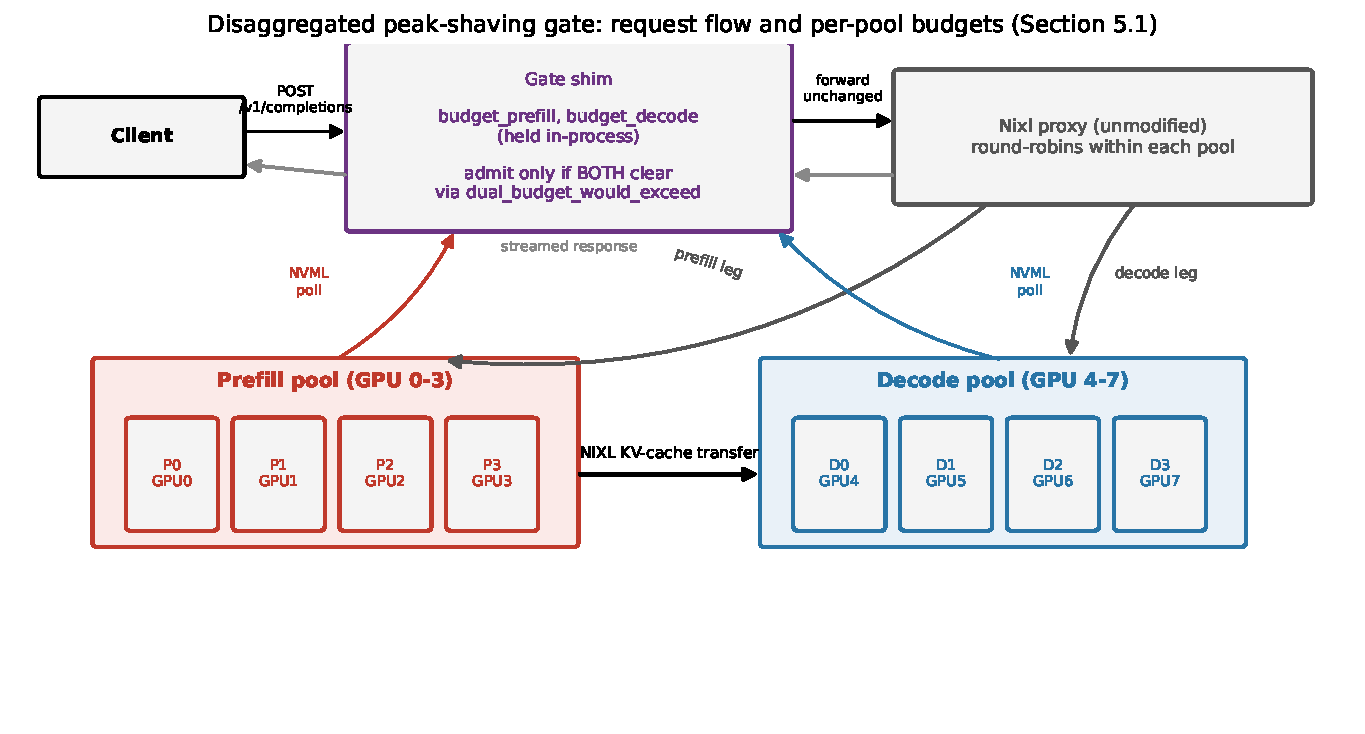
\includegraphics[width=\linewidth]{figs/architecture.pdf}
  \caption{Request flow through the gate shim, Nixl proxy, and both pools, and where each
    pool's \texttt{PowerBudget} gets its power samples from.}
  \label{fig:architecture}
\end{figure}

\subsection{Baseline and gated result ($n{=}3$)}
\label{sec:baseline-gated}

An uncapped baseline on this topology (first measurement at 4:4 scale) shows the decode pool
drawing \emph{more} sustained power than the prefill pool (895.4~W vs.\ 587.8~W mean, first
trial) --- four decode instances are continuously batch-decoding for the whole trial, while
four prefill instances draw power only in short bursts per admitted request. With each pool's
cap set to 92.5\% of its own measured mean (mirroring the colocated gate's own cap/mean ratio
for comparable aggressiveness), replicated $n{=}3$ (mean $\pm$ population std across trials):

\begin{table}[t]
  \caption{Closed-loop, 92.5\%-of-mean cap, $n{=}3$. Max windowed-average (15~s) peak power
    per pool, baseline vs.\ gated.}
  \label{tab:baseline-gated}
  \footnotesize
  \begin{tabular}{@{}lrrr@{}}
    \toprule
    Pool & Baseline & Gated & Reduction \\
    \midrule
    Prefill & $1121.2{\pm}11.1$~W & $919.0{\pm}20.8$~W & $\mathbf{18.0\%}$ \\
    Decode  & $1210.0{\pm}3.5$~W  & $1187.3{\pm}5.1$~W & $\mathbf{1.9\%}$ \\
    \bottomrule
  \end{tabular}
\end{table}

The gap between conditions is large relative to across-trial noise for both pools (prefill: a
202~W gap against $\leq$21~W std, roughly 10 std devs; decode: a 23~W gap against $\leq$5~W
std, roughly 4--6 std devs) --- the asymmetry is not an $n{=}1$ artifact. Mean TTFT:
$1.770{\pm}0.075$~s (baseline) $\rightarrow$ $10.951{\pm}0.168$~s (gated), a $+9.18$~s cost,
also tight across trials.

For comparison, the colocated gate's single combined budget achieved ${\sim}7$--8\% at a
comparable cap ratio (\S\ref{sec:crosspolicy}) --- the disaggregated design's prefill-pool
result clearly exceeds it, at a comparable-or-smaller absolute TTFT cost ($+9.18$~s here
vs.\ the colocated result's roughly $+11$ to $+14.5$~s). But the decode-pool result is far
below it. \textbf{The value of per-pool budgets is not (only) that they beat the colocated
number --- it is that they reveal that the colocated gate's apparent effectiveness is really
prefill-driven, with decode along for the ride}, a distinction a single combined fleet number
cannot expose.

\subsection{Why: a controlled concurrency sweep}
\label{sec:concurrency}

To test whether this asymmetry is really about admission gating's structural inability to
touch already-running streams (our working hypothesis), rather than some other artifact, we
ran a dedicated spike: hold a single decode instance at fixed, controlled concurrency levels
(2, 8, 32 concurrent decode streams, short uniform prompts, fixed 512-token cap) and measure
steady-state decode-GPU power at each level.

\begin{table}[t]
  \caption{Decode-GPU power vs.\ controlled concurrency, $n{=}1$ (single dedicated instance).}
  \label{tab:concurrency}
  \footnotesize
  \begin{tabular}{@{}lrr@{}}
    \toprule
    Concurrency & Mean decode power & $\Delta$ vs.\ previous \\
    \midrule
    0 (idle) & 40.5~W  & --- \\
    2        & 273.8~W & $+233.3$~W \\
    8        & 282.0~W & $+8.2$~W \\
    32       & 309.5~W & $+27.5$~W \\
    \bottomrule
  \end{tabular}
\end{table}

Going from zero active streams to just two already captures 88\% of the total power range
observed across the entire sweep; a further $16\times$ increase in concurrency
($2\rightarrow32$) adds only 13\% more power. Decode power is not proportional to concurrent
load --- it is dominated by whether the GPU is doing decode work \emph{at all}. This directly
explains \S\ref{sec:baseline-gated}'s result: in a workload where the decode pool is rarely
fully idle, admission gating can only ever move concurrency within the flat part of this
curve; it never gets the chance to push power toward the much lower idle floor, where the
real headroom is. It also directly implies a limit on what \emph{any} admission-side
mechanism (including shedding or concurrency caps) could achieve on the decode side without
idling instances outright --- a materially different, larger mechanism than admission
control, which we leave to future work.

\subsection{The prefill-side power/latency tradeoff}
\label{sec:tradeoff}

Unlike decode, the prefill-side effect is a genuine, tunable tradeoff. A 4-point closed-loop
cap sweep (no-gate, and caps at 92.5\%, 80\%, and 65\% of the prefill pool's own uncapped
mean) shows a clean, monotonic relationship between cap aggressiveness, mean request latency,
and achieved peak-power reduction. The no-gate and 92.5\% points are the $n{=}3$ replicated
values from \S\ref{sec:baseline-gated}; the 80\% and 65\% points are $n{=}1$ (not yet
replicated --- see \S\ref{sec:discussion}):

\begin{table}[t]
  \caption{Closed-loop gating-intensity sweep, prefill pool (see Table~\ref{tab:decode-sweep}
    for the corresponding decode-pool numbers at each intensity).}
  \label{tab:prefill-sweep}
  \footnotesize
  \begin{tabular}{@{}lrrrr@{}}
    \toprule
    Cap (\% of mean) & Mean TTFT & Mean TPOT & Prefill max windowed & Reduction \\
    \midrule
    No-gate ($n{=}3$) & 1.77~s  & 18.15~ms & 1121.2~W & --- \\
    92.5\% ($n{=}3$)  & 10.95~s & 17.57~ms & 919.0~W  & 18.0\% \\
    80\% ($n{=}1$)    & 13.78~s & 17.47~ms & 817.7~W  & 27.7\% \\
    65\% ($n{=}1$)    & 20.91~s & 17.24~ms & 736.1~W  & 34.9\% \\
    \bottomrule
  \end{tabular}
\end{table}

Pushing the cap from 92.5\% to 65\% of mean roughly doubles the achievable peak-power
reduction at the cost of roughly doubling mean TTFT --- a real, operator-tunable dial. Mean
TPOT is essentially unaffected by gating intensity throughout (17.2--18.2~ms across every
point): the gate controls \emph{when} a request is admitted, not how fast it decodes once
started, so TTFT --- not TPOT --- is the metric that actually reflects the gate's cost. The
decode pool's corresponding sweep, by contrast, is flat --- consistent with
\S\ref{sec:concurrency}'s explanation and shown alongside the prefill curve in
Figure~\ref{fig:tradeoff}:

\begin{table}[t]
  \caption{Closed-loop gating-intensity sweep, decode pool. 92.5\% row uses the $n{=}3$ value
    (Table~\ref{tab:baseline-gated}); no-gate/80\%/65\% use each condition's own $n{=}1$
    trial, compared against that same trial's paired baseline for consistency.}
  \label{tab:decode-sweep}
  \footnotesize
  \begin{tabular}{@{}lrr@{}}
    \toprule
    Cap (\% of mean) & Decode max windowed & Reduction \\
    \midrule
    No-gate          & 1205.2~W & --- \\
    92.5\% ($n{=}3$) & 1187.3~W & 1.9\% \\
    80\%             & 1190.8~W & 1.2\% \\
    65\%             & 1186.8~W & 1.5\% \\
    \bottomrule
  \end{tabular}
\end{table}

\begin{figure}[t]
  \centering
  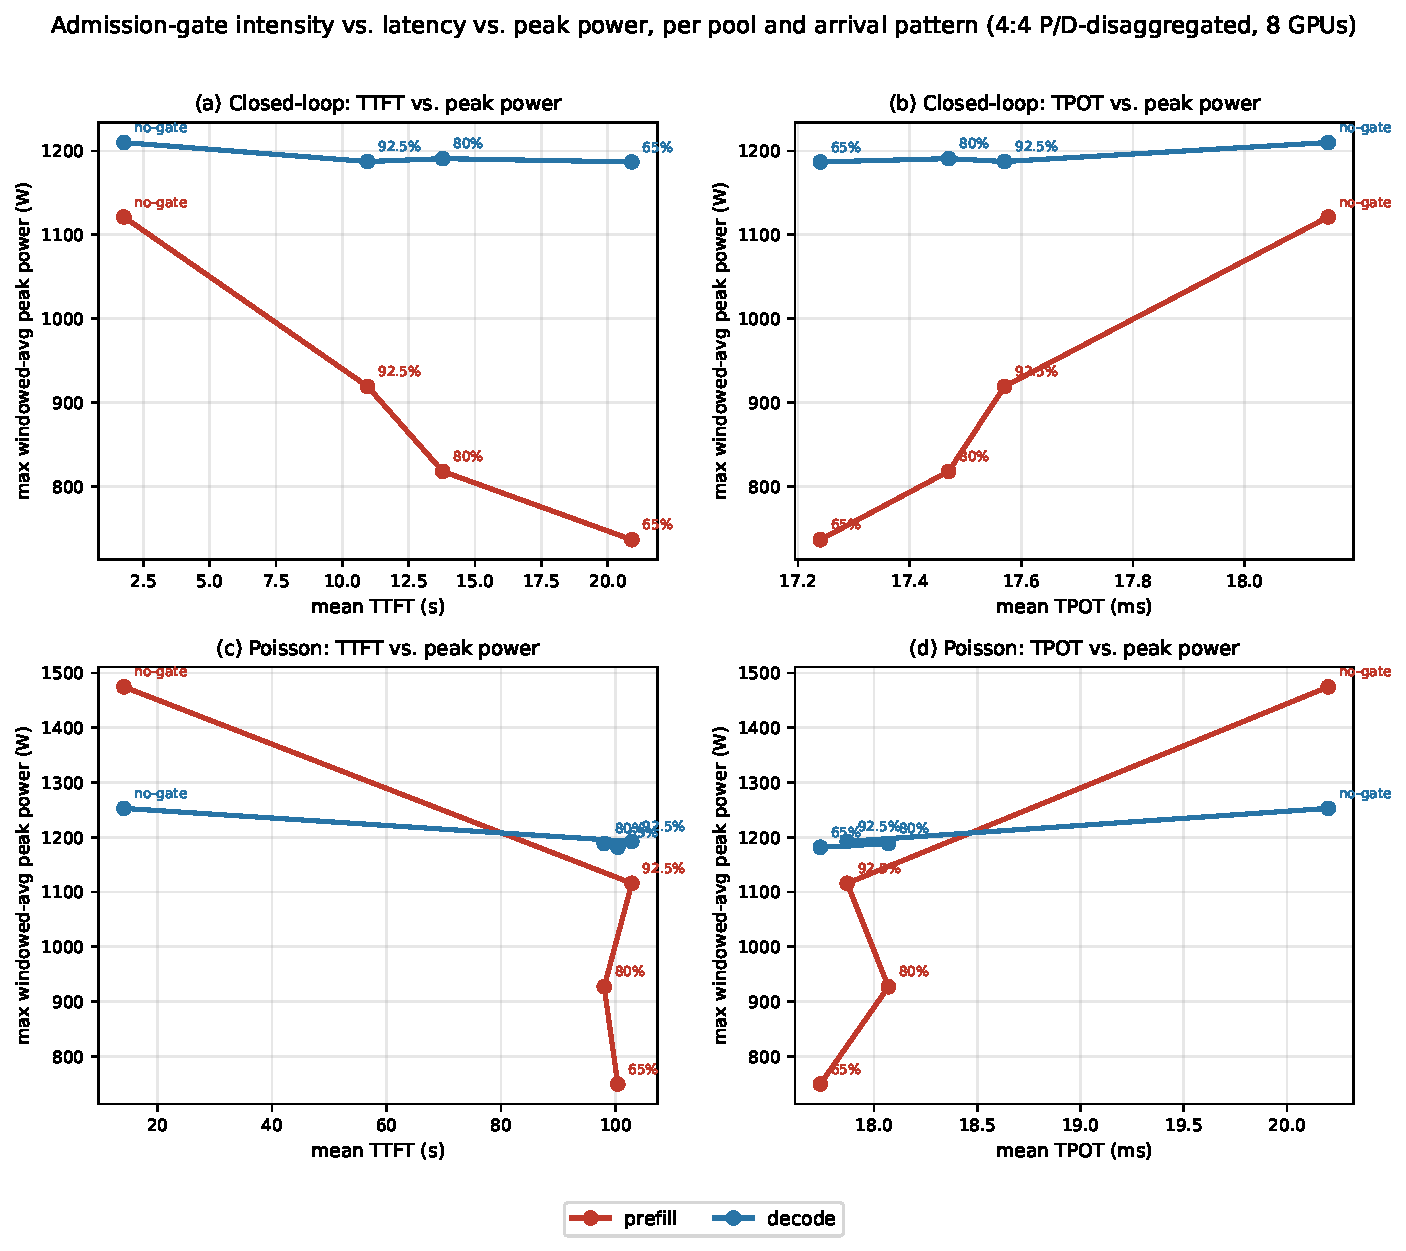
\includegraphics[width=\linewidth]{figs/gating_tradeoff.pdf}
  \caption{$2{\times}2$ grid --- (a)/(b) closed-loop TTFT/TPOT vs.\ max windowed-average peak
    power (Tables~\ref{tab:prefill-sweep}--\ref{tab:decode-sweep}), (c)/(d) the same for
    Poisson arrivals (Tables~\ref{tab:poisson}, \ref{tab:poisson-sweep}, \S\ref{sec:poisson}),
    plotted with independent axis scaling per row since Poisson's TTFT range is
    $5$--$10\times$ closed-loop's.}
  \label{fig:tradeoff}
\end{figure}

\subsection{Robustness to arrival pattern, and a harness bug worth reporting}
\label{sec:poisson}

We repeated the no-gate/92.5\%-cap pair under open-loop Poisson arrivals (rate matched to
this project's established closed-loop-vs-open-loop ``Matched'' condition convention),
replicated $n{=}3$, to check whether the asymmetry is an artifact of closed-loop arrival
control specifically.

\begin{table}[t]
  \caption{Poisson open-loop arrivals, 92.5\%-of-mean cap, $n{=}3$ (same cap as
    Table~\ref{tab:baseline-gated}).}
  \label{tab:poisson}
  \footnotesize
  \begin{tabular}{@{}lrrr@{}}
    \toprule
    Pool & Poisson baseline & Poisson gated & Reduction \\
    \midrule
    Prefill & $1474.5{\pm}26.3$~W & $1115.8{\pm}39.0$~W & $\mathbf{24.3\%}$ \\
    Decode  & $1252.6{\pm}10.2$~W & $1192.2{\pm}3.0$~W  & $\mathbf{4.8\%}$ \\
    \bottomrule
  \end{tabular}
\end{table}

The qualitative finding replicates cleanly --- prefill shaves far more than decode under
Poisson arrivals too, and by a consistently larger margin than closed-loop's 18.0\%/1.9\%
(\S\ref{sec:baseline-gated}), across all 3 trials. But the \emph{cost} differs sharply: mean
TTFT rises from $14.154{\pm}0.872$~s to $102.856{\pm}4.759$~s (vs.\ $1.770$~s
$\rightarrow$ $10.951$~s at the same cap under closed-loop) --- roughly $+88.7$~s under
Poisson against $+9.18$~s under closed-loop, a ${\sim}10\times$ gap that holds across all 3
replicate pairs, not just the first trial.

The failure rate under gated Poisson arrivals is itself noticeably noisy trial-to-trial ---
14, 54, and 43 of 750 requests failed outright (1.9\%, 7.2\%, 5.7\%) across the 3 trials, even
against a 300~s client-side timeout --- and this interacts with how $\mathit{mean\_ttft}$
should be read: a failed request is excluded from the mean (it has no measured TTFT), so a
trial with more failures is also a trial where more of the worst-tail cases were removed from
the average rather than included as large values --- the trial with the most failures (54)
shows the \emph{lowest} mean TTFT of the three (96.3~s) for exactly this reason, not because
that trial was actually less congested. We report $\mathit{mean\_ttft}$ here as a
success-conditional statistic and flag this explicitly rather than let it read as a directly
comparable central tendency across trials with different failure rates.

\textbf{The same cap is not equally aggressive across arrival patterns} --- Poisson's
burstier arrivals can spike demand in ways a closed-loop concurrency ceiling structurally
prevents, so cap selection needs to account for the arrival process, not just sustained mean
power, echoing a pattern we also observed in the colocated gate's own open-loop validation
(\S\ref{sec:bugs}).

\textbf{Extending to the full 4-point sweep sharpens this into something stronger than a
caveat: it is a genuine breakdown, not just a cost.} We reran the 80\% and 65\% closed-loop
cap values (same absolute Watts, 470~W/716~W and 382~W/582~W) under Poisson arrivals,
$n{=}1$ each:

\begin{table}[t]
  \caption{Poisson gating-intensity sweep, prefill pool (92.5\% row is $n{=}3$,
    Table~\ref{tab:poisson}; others $n{=}1$). \texttt{n\_failed} is now the load-bearing
    column.}
  \label{tab:poisson-sweep}
  \footnotesize
  \begin{tabular}{@{}lrrrr@{}}
    \toprule
    Cap (\% of mean) & Mean TTFT & $n_\mathit{failed}$/750 & Prefill max windowed & Reduction \\
    \midrule
    No-gate ($n{=}3$) & 14.15~s  & 2 (0.3\%)          & 1474.5~W & --- \\
    92.5\% ($n{=}3$)  & 102.86~s & avg 37 (4.9\%)      & 1115.8~W & 24.3\% \\
    80\%              & 98.02~s  & 84 (11.2\%)         & 926.8~W  & 37.1\% \\
    65\%              & 100.40~s & 229 (\textbf{30.5\%}) & 749.0~W  & 49.2\% \\
    \bottomrule
  \end{tabular}
\end{table}

\begin{table}[t]
  \caption{Poisson gating-intensity sweep, decode pool.}
  \label{tab:poisson-sweep-decode}
  \footnotesize
  \begin{tabular}{@{}lrr@{}}
    \toprule
    Cap (\% of mean) & Decode max windowed & Reduction \\
    \midrule
    No-gate          & 1252.6~W & --- \\
    92.5\% ($n{=}3$) & 1192.2~W & 4.8\% \\
    80\%             & 1188.4~W & 5.1\% \\
    65\%             & 1181.6~W & 5.7\% \\
    \bottomrule
  \end{tabular}
\end{table}

Taken at face value, the prefill trend ($24.3\%\rightarrow37.1\%\rightarrow49.2\%$) looks
like the closed-loop tradeoff continuing to scale cleanly. It does not.
\textbf{$\mathit{mean\_ttft}$ is flat (98--103~s) across all three capped points instead of
climbing} --- the opposite of closed-loop's clean monotonic rise
(Table~\ref{tab:prefill-sweep}). This is the same success-conditional-statistic effect from
above, now dominating the picture: as the cap tightens, a growing share of requests stop
waiting and start failing outright ($4.9\%\rightarrow11.2\%\rightarrow30.5\%$) rather than
completing at ever-larger TTFT, so the survivors' mean TTFT stops moving even though the
underlying congestion keeps getting worse. \textbf{The 65\% Poisson point is not really
``49.2\% peak-power reduction at ${\sim}100$~s mean TTFT'' --- it is ``49.2\% peak-power
reduction achieved partly by silently failing to serve nearly a third of requests.''} We do
not read this as the mechanism scaling gracefully to more aggressive caps; we read it as the
same structural limit as \S\ref{sec:limit}'s engineered worst-case burst, now reached by a
different route (bursty arrivals rather than a single large burst), and worth reporting
exactly as bluntly as the numbers show it.

Diagnosing this cleanly required fixing a real bug in our own measurement harness first: the
open-loop arrival code path spawned each simulated conversation as a bare, unguarded thread,
and a request that exceeded the client-side socket timeout under heavy admission delay raised
an exception type (\texttt{TimeoutError}) that was not caught anywhere in that code path ---
the thread died silently, and the conversation never appeared in the output at all (not even
as a recorded failure). This affected roughly 11\% of requests in our first attempt at the
gated Poisson condition specifically (the only condition with wait times long enough to
trigger it) and would have understated both the true tail latency and the true failure rate
had we not caught it --- the reported numbers above are from the corrected run, verified to
show zero silently-dropped requests. We report this because the diagnostic pattern (a
systematic result looks anomalous $\rightarrow$ trace it to a specific, fixable measurement
bug $\rightarrow$ fix and re-validate) is the same one that produced every other finding in
this paper, and we think it is worth making visible rather than only fixing quietly.

\subsection{Electricity-cost implications, and why this estimate is preliminary}
\label{sec:cost}

Everything reported so far is a per-pool peak --- prefill's 15~s max windowed-average and
decode's, measured separately (Tables~\ref{tab:baseline-gated}, \ref{tab:poisson}). A real
demand charge does not bill per pool: it bills on the facility's \emph{combined} draw, the
highest average power the whole site pulls during any one interval of the billing period,
typically 15 minutes for commercial and industrial customers in the U.S., at rates commonly
\$5--30/kW-month and accounting for 30--70\% of the total electric bill
\cite{mclaren2017demandcharges}. So the number that matters for a cost argument is not the
per-pool figures but the \emph{sum} of both pools' power at each instant, windowed and maxed
the same way.

We recomputed this combined series for the closed-loop flagship comparison ($n{=}3$, 92.5\%
cap, same trials as Table~\ref{tab:baseline-gated}) by merging the independently-timestamped
prefill and decode power-logger CSVs into 1-second bins (averaging, not summing, samples within
each bin --- an early version of this analysis summed instead and produced a fleet power figure
of ${\sim}21$~kW for hardware whose $8\times450$~W-TDP maximum is under 4~kW, a bug we caught
by that exact sanity check before it went any further) and applying the same 15-second
max-windowed-average as everywhere else.

\begin{table}[t]
  \caption{Facility-wide (combined prefill+decode) power, closed-loop, $n{=}3$.}
  \label{tab:combined-power}
  \footnotesize
  \begin{tabular}{@{}lrr@{}}
    \toprule
    Condition & Combined mean power & Combined 15~s max windowed-avg \\
    \midrule
    No-gate            & $1507.5\pm13.6$~W & $2275.1\pm14.2$~W \\
    Gated (92.5\%)     & $1186.9\pm11.4$~W & $1993.8\pm37.8$~W \\
    \textbf{Reduction} & \textbf{21.3\%}    & \textbf{12.4\%} \\
    \bottomrule
  \end{tabular}
\end{table}

The facility peak drops 281~W ($2275\rightarrow1994$~W) --- smaller than either pool's own
percentage reduction (\S\ref{sec:baseline-gated}'s 18.0\%/1.9\%) because the two pools' peaks
do not occur at exactly the same instant, so the combined peak is not simply the sum of the two
individual peaks. At \$5--30/kW-month, that reduction is worth \$1.41--\$8.44/month for this
one 8-GPU node. Read as an absolute number this is negligible; read as a 12.4\% reduction in
the demand-charge component of a much larger fleet's bill (which scales with node count if
peaks are independent across nodes, though coincidence effects across a real fleet would need
their own accounting, not simply per-node multiplication) it is the more meaningful framing,
and matches the \emph{relative} language we use for every other result in this paper.

\textbf{This estimate should be read as preliminary, for a specific reason the numbers above
expose directly.} A real demand charge bills on a 15-\emph{minute} average; our measurement
uses a 15-\emph{second} window, and our entire battery only runs 200--380 seconds end to end
(\S\ref{sec:baseline-gated}) --- roughly 15--25$\times$ shorter than even one real billing
interval. A peak sustained for 15 seconds inside a 15-minute averaging window is diluted by a
factor of up to 60 before it reaches the utility's meter; whether our demonstrated \emph{shape}
of reduction survives that dilution, shrinks toward zero, or (if the gate's effect is not a
brief transient but persists across a full 15-minute load profile) holds up close to unchanged,
is exactly the open question a longer, multi-window-length trial (15~s/1~min/5~min/15~min)
would answer, and is not something this short-battery result can resolve on its own.

\section{Discussion and Limitations}
\label{sec:discussion}

\textbf{Statistical rigor.} The two flagship comparisons --- closed-loop and Poisson, each
no-gate/92.5\%-cap (\S\ref{sec:baseline-gated} and \S\ref{sec:poisson}) --- are now
replicated $n{=}3$, and the core asymmetry (prefill shaves far more than decode) holds well
outside across-trial noise in both: a 10-std-dev gap for prefill and a 4--6-std-dev gap for
decode under closed-loop, and a consistent ordering across all 3 trials under Poisson. The
arrival-pattern latency-cost gap (${\sim}9.2$~s vs.\ ${\sim}88.7$~s at the same cap) is
likewise stable across all 3 replicate pairs. The gating-intensity sweep's other three points
per arrival pattern (closed-loop 80\%/65\%, Poisson 92.5\%/80\%/65\% beyond the $n{=}3$
92.5\% point --- \S\ref{sec:tradeoff}, \S\ref{sec:poisson}) and the concurrency sweep
(\S\ref{sec:concurrency}) remain $n{=}1$, providing \emph{robustness} evidence --- the same
qualitative finding holding across a range of caps --- rather than statistical replication;
extending $n{=}3$ to those points is the natural next step if reviewers want the full
tradeoff curve, not just its endpoints, replicated. The Poisson-gated failure rate is itself
a source of real, non-trivial variance that grows with cap aggressiveness --- 1.9--7.2\%
trial-to-trial at the 92.5\% cap alone ($n{=}3$), rising to 11.2\% at 80\% and 30.5\% at 65\%
(both $n{=}1$) --- which we report explicitly rather than average away, and which at 65\% is
large enough that the reported peak-power reduction should be read as partly a
shedding-by-failure artifact, not pure admission-pacing (\S\ref{sec:poisson}).

\textbf{Comparison fairness.} The colocated-vs-disaggregated comparison
(\S\ref{sec:baseline-gated}) is not matched in scale --- six homogeneous replicas vs.\
four-and-four disaggregated pools --- so ``disaggregation beats colocation'' is not quite the
claim we make; ``disaggregation reveals where the mechanism actually works'' is the
defensible one, and is what we argue throughout.

\textbf{Decode-side peak shaving remains unsolved.} \S\ref{sec:concurrency}'s mechanistic
result implies that meaningfully shaving decode-pool peak power requires periodically idling
or draining decode instances entirely, not admission-side throttling of any kind --- a
materially different, larger system than anything this paper builds. We consider this the
natural next step for this line of work.

\textbf{Electricity-cost estimate is a preliminary, short-window proxy.} \S\ref{sec:cost}'s
demand-charge savings figure is computed from a 15-second max windowed-average over a
200--380-second battery, while real demand charges bill on a 15-\emph{minute} average ---
roughly a $60\times$-longer averaging window than we measure, over a billing period our short
batteries do not come close to spanning. We report the estimate because the underlying
combined-power numbers are real and the framing is directly relevant to the gate's stated
motivation, but we do not yet know whether the percentage reduction holds, shrinks, or grows
once measured at the window length and duration that determines an actual utility bill; a
longer multi-window-length trial (\S\ref{sec:cost}) is needed before this number should be
treated as more than illustrative.

\textbf{Scope.} Single 8-GPU box, one 7B model, one workload family (ShareGPT-derived
conversational traffic with a whale-injection long-prompt mix), a fixed 4:4 prefill:decode
ratio not independently tuned for this workload. Generalization across model scale, hardware
topology, and prefill:decode provisioning ratio is untested.

\section{Conclusion}

We show that a peak-shaving admission gate --- deferring, not shedding, requests to stay
under a rolling-window power cap with no physical energy storage --- works on real hardware,
and that applying it to real prefill/decode-disaggregated serving with independent per-pool
budgets does more than match a colocated design: it reveals a genuine,
mechanistically-explained asymmetry in where the mechanism actually has leverage. Admission
gating is a real, tunable lever for prefill-pool peak power and essentially not one for
decode-pool peak power, because decode power is dominated by already-running work that
admission control cannot retroactively touch. We view this as a stronger and more actionable
result than a single aggregate effectiveness number would have been: it tells a deployment
exactly which knob to turn, and exactly what a different mechanism would need to address
next.

\bibliographystyle{ACM-Reference-Format}
\bibliography{references}

\end{document}
